\chapter{Plane algebraic curves}
\epigraph[author={Felix Klein}]{Everyone knows what a curve is, until he has studied enough mathematics to become confused through the countless number of possible exceptions.}\SubIndex{Klein, Felix}
\section{Example}\label{example:rational.cubic}
Let's find the solutions of the algebraic equation \(y^2=x^2+x^3\).
The solutions form a curve in the plane, intuitively because the equation is one constraint on two variables.
There is one obvious solution: \((x,y)=(0,0)\).
A minor miracle: almost every line through \((0,0)\) passes through another point of the curve, which we can compute.
To see this, write any line through \((0,0)\), say with slope \(t\), as \(y=tx\).
Plug this in to the equation \(y^2=x^2+x^3\) to see if we can find any more solutions:
\[
(tx)^2=x^2+x^3,
\]
which we simplify to get either \(x=0\) or, dividing by \(x^2\),
\[
t^2=1+x.
\]
Solving for \(x\), we find \(x=t^2-1\).
Plug in to the equation of the line \(y=tx\) to get \(y=t\pr{t^2-1}\).
Every solution, except \((x,y)=(0,0)\), has to lie on some line through \((0,0)\), and that line will be either \(y=tx\) or a vertical line \(x=0\).
But on the line \(x=0\), the only solution is \(y=0\), the origin.
Moreover, if we let \(t=\pm 1\), we get the solution \((x,y)=(0,0)\) too.
So we get all of the solutions.
{%\begin{center}
\pgfplotsset{compat=1.12,width=7cm}%
\inputinexample{cubic-curve-2}
}%\end{center}
Each line strikes the curve at two points (one of which is the origin); except for the vertical line.
\begin{problem}{intersecting.curves:other.cubic}
Prove that every point \((x,y)\) on the curve \(x^3=y(x+y)\) has the form \(x=t+t^2\), \(y=t(t+t^2)\) for some \(t\).
\end{problem}
\begin{problem*}{algebraic.curves:n.n.minus.1}
Take an algebraic curve \(0=p(x,y)\), where \(p(x,y)\) is a sum of terms of degree \(n-1\) or \(n\).
Prove that by substituting \(y=tx\) as above, we can solve for \(x,y\) as functions \(x=x(t), y=y(t)=tx(t)\).
\end{problem*}
\section{Definition}
A \emph{plane algebraic curve}\define{curve!plane algebraic}\define{plane algebraic!curve} is the set of zeroes of a nonconstant polynomial in two variables; the \emph{degree}\define{degree!of algebraic curve}\define{curve!degree} of the curve is the degree of the polynomial.
\[
\begin{array}{@{}r>{$}l<{$}}
\toprule
\text{degree}&\text{appellation}\\
\cmidrule(r){1-1}\cmidrule(l){2-2}
1&line\define{line}\\
2&conic\define{conic}\\
3&cubic\define{cubic!curve}\define{curve!cubic}\\
4&quartic\define{curve!quartic}\define{quartic!curve}\\
5&quintic\define{curve!quintic}\define{quintic!curve} \\
6&sextic\define{curve!sextic}\define{sextic!curve} \\
7&septic\define{curve!septic}\define{septic!curve} \\
8&octic\define{curve!octic}\define{octic!curve} \\
\bottomrule
\end{array}
\]
\begin{problem}{algebraic.curves:ptolemy}
Use the same trick for the circle \(x^2+y^2=1\) as follows.
Show first (using the formula for the slope of a line) that for any point \((x,y)\) of the circle, the line through \((0,1)\) and \((x,y)\) passes through the horizontal axis at the point \((t,0)\) where
\[
t=\frac{x}{1-y}.
\]
It helps to draw a picture.
Solve for \(x\): \(x=t(1-y)\), and plug into the equation of the circle to find that 
\[
\pr{x,y}=\frac{1}{t^2+1}\pr{2t,t^2-1}.
\]
Explain now why every rational point of the circle corresponds to a rational value of \(t\) and vice versa.
Explain why the same conclusion holds over any field \(k\).
\end{problem}
\begin{example}
Let's try a different cubic curve.
Take the cubic curve
\[
y^2=(x+1)x(x-1).
\]
{%\begin{center}
\pgfplotsset{compat=1.12,width=7cm}%
\inputinexample{cubic-curve-3}
}%\end{center}
We see right away that some lines strike the curve in more than two points, one at the origin, and two others.
Calculate as above that those two others are
\[
x=\frac{t^2\pm \sqrt{t^4+4}}{2}, \ y=tx.
\]
\end{example}

\begin{example}
Fermat's Last Theorem\define{Fermat's Last Theorem} says that there are no integer solutions to \(a^n+b^n=c^n\) with nonzero integers \(a,b,c\) and \(n\ge 3\).
Dividing both sides by \(c\), if there were a solution, we would solve 
\[
x^n+y^n=1
\]
with nonzero rational numbers \(x,y\).
Conversely, any nonzero rational numbers \(x,y\) solving this equation, after clearing denominators, give a solution to \(a^n+b^n=c^n\).
So Fermat's Last Theorem is equivalent to the statement that the plane algebraic curve \(x^n+y^n=1\) has no rational number solutions except \((x,y)=(0,1), (0,-1), (1,0)\) and \((-1,0)\).
In particular, we are interested in plane algebraic curves over the rational numbers, not just the real numbers.
\end{example}
\begin{example}
Looking for integer solutions of integer polynomial equations, we can look at those equations modulo a prime, and get equations over a finite field. 
So it is natural to consider algebraic curves over any field.
\end{example}
\begin{example}
Consider the polynomial equation \(x^2+y^2=-7\).
There are no real values of \(x,y\) that satisfy this, so the algebraic curve is empty.
\end{example}
To remedy this problem, we allow the variables \(x\) and \(y\) to take on complex values.
Sticking in a value for one of the variables, or perhaps for the other, with a suitable choice of value, we will find that we have a nonconstant polynomial in one variable, so there is a solution \((x,y)\) by the fundamental theorem of algebra.
Hence algebraic curves have complex points, but perhaps no real points.

Take a field \(k\) and an algebraic closure \(k\subset \bar{k}\).
A \emph{plane algebraic curve} \(C\) over \(k\) given by a nonconstant polynomial equation \(f(x,y)=0\) with coefficients in \(k\) is the set \(C\) of its \(\bar{k}\)-points, i.e. points \((x,y)\) with \(x,y\) in the algebraic closure \(\bar{k}\) satisfying \(f(x,y)=0\).
\begin{problem}{algebraic.curves:k.bar.points}
Prove that there are infinitely many \(\bar{k}\)-points on any plane algebraic curve over \(k\).
\end{problem}
The equation of an algebraic curve is not uniquely determined.
The curve \(x^2-y=0\) is the same curve as \(\pr{x^2-y}^9=0\).
The curve \(xy=0\) splits into \(x=0\) or \(y=0\), two curves.
If the equation of a curve has nonconstant factors, we say that the curve is \emph{reducible}% 
\define{irreducible!curve}%
\define{reducible!curve}% 
\define{curve!irreducible}%
\define{curve!reducible} 
and the equations formed from the factors, or the curves they cut out, are \emph{components}\define{component} of the curve.
We can assume that the polynomial \(f(x,y)\) in the equation \(f(x,y)=0\) of a curve is not a square, cube, etc. of any polynomial, nor a constant multiple of a square, cube, etc.
\begin{problem}{plane.algebraic.curves:line.intersection}
Suppose that \(C\) is a plane algebraic curve of degree \(d\).
Prove that every line in the plane that intersects \(C\) more than \(d\) times, in the algebraic closure of the field, is a component of \(C\).
\end{problem}
\begin{answer}{plane.algebraic.curves:line.intersection}
We can replace our field by its algebraic closure without affecting the result, so suppose that the field is algebraically closed.
By linear change of variables, arrange that the line is \(y=0\).
Then the equation \(0=p(x,y)\) of our curve \(C=(0=p(x,y))\) becomes \(0=p(x,0)\), of degree at most \(d\), or else there is a factor of \(y\) in \(p(x,y)\), i.e. \(C\) is reducible with our line as a component.
\end{answer}
\begin{lemma}
An irreducible plane algebraic curve determines its equation uniquely up to scaling by a nonzero constant.
\end{lemma}
\begin{proof}
Work over a field \(k\) with algebraic closure \(\bar{k}\).
Take two irreducible equations \(0=b(x,y)\) and \(0=c(x,y)\) with the same curve, i.e. the same points over \(\bar{k}\).
For any constant \(x=a\) over \(\bar{k}\), the equations \(0=b(a,y)\) and \(0=c(a,y)\) have the same solutions.
Unless the \(x\) variable does not appear in either equation, these are infinitely many different points in common on the curve.
But if \(x\) does not appear, swap \(x\) with \(y\) and repeat.
By proposition~\vref{proposition:resultant.degree}, \(b(x,y)\) and \(c(x,y)\) have a common factor.
\end{proof}

\section{Regular morphisms}
A \emph{regular function}\define{regular!function}\define{function!regular} on a plane algebraic curve is the restriction of a polynomial function.
\begin{example}
On the plane algebraic curve \((y^2=x^2+x^3)\), the functions \(y^2\) and \(x^2+x^3\) take on the same values at every point, and therefore are the same regular function.
\end{example}
\begin{example}
On the hyperbola \((1=x^2-y^2)\), note that \((x-y)(x+y)=x^2-y^2=1\), so \(1/(x-y)\) at first sight doesn't look regular, but \(1/(x-y)=x+y\) is clearly regular on the hyperbola.
\end{example}
If \(C\) is a plane algebraic curve over field \(k\), let \(k[C]\) be the set of regular functions on \(C\) with coefficients in \(k\); clearly \(k[C]\) is an algebra over \(k\).

A \emph{regular morphism}\define{morphism!regular} of plane algebraic curves \(f \colon C \to D\) is a map which can be expressed somehow as \(f(x,y)=(s(x,y),t(x,y))\) for two polynomials \(s(x,y), t(x,y)\), so that \(f\), applied to any point of \(C\), yields a point of \(D\).
\begin{example}
The map \(f(x,y)=(s,t)=\pr{x^2-2,x(x^2-1)}\) maps \(C=(y=0)\) to \(D=(t^2=s^2+s^3)\), as we saw previously.
\end{example}
A regular morphism with an inverse regular morphism is \emph{biregular}\define{biregular}, and the associated curves are \emph{biregular}.
Clearly biregular plane algebraic curves have isomorphic algebras of regular functions.
\begin{example}
The map \(f(x,y)=(s,t)=\pr{x,x^2}\) maps the line \(C=(x=y)\) to the parabola \(D=(t=s^2)\), with inverse \(g(s,t)=(x,y)=(s,s)\).
These maps are not inverses of one another in the plane, but they invert one another along the curves \(C\) and \(D\) in the plane.
\end{example}
\begin{problem}{plane.algebraic.curves:ellipses}
Prove that the ellipses \(x^2+y^2=a^2\), for any real constant \(a>0\), are biregular as real plane algebraic curves.
\end{problem}
\begin{problem}{plane.algebraic.curves:inverse.morphism}
Prove that every isomorphism of algebras of regular functions of irreducible plane algebraic curves arises uniquely from a biregular morphism. 
\end{problem}
\begin{answer}{plane.algebraic.curves:inverse.morphism}
Suppose that \(C\) has equation \(c(x,y)=0\) and \(D\) has equation \(d(s,t)=0\).
Take an algebra isomorphism \(\Phi\colon k[C]\to k[D]\).
This map \(\Phi\) is uniquely determined by \(\Phi(x),\Phi(y)\), because after that every polynomial \(f(x,y)\) is mapped to \(\Phi(f(x,y))=f(\Phi(x),\Phi(y))\), as the algebra morphism preserves the addition and multiplication operations by which we construct polynomials.
Pick polynomials \(x(s,t),y(s,t)\) so that, in \(k[D]\), \(x(s,t)=\Phi(x)\) and \(y(s,t)=\Phi(y)\).
Let
\[
\psi\colon (s,t)\in\bar{k}^2\mapsto(x,y)=(x(s,t),y(s,t))\in\bar{k}^2.
\]
Two polynomials agree along the \(\bar{k}\)-points of the curve \(D\) just when their difference vanishes at those points, so just when their difference is divisible by \(d(s,t)\), by irreducibility of \(d(s,t)\).
So these \(x(s,t),y(s,t)\) are determined only up to multiples of the irreducible \(d(s,t)\).

Since \(\Phi\) is an isomorphism, it has an inverse isomorphism \(\Phi^{-1}\), and so we can similarly find polynomials \(s(x,y),t(x,y)\), defined up to adding multiples of \(c(x,y)\), so that \(s(x,y)=\Phi^{-1}s,t(x,y)=\Phi^{-1}t\) in \(k[C]\).
Define a map
\[
\varphi\colon (x,y)\in\bar{k}^2\mapsto(s,t)=(s(x,y),t(x,y))\in\bar{k}^2.
\]
Extend \(\Phi\) to a map \(k[x,y]\to k[s,t]\) by 
\[
\Phi(x)=x(s,t), \Phi(y)=y(s,t)
\]
and similarly extend \(\Phi^{-1}\) to a map \(\Psi\colon k[s,t]\to k[x,y]\) by 
\[
\Psi(s)=s(x,y), \Psi(t)=t(x,y).
\]

On any polynomial \(f(x,y)\),
\begin{align*}
f(\psi(s,t))
&=
f(x(s,t),y(s,t)),
\\
&=
f(\Phi(x),\Phi(y)),
\\
&=
\Phi(f(x,y)).
\end{align*}
Similarly, for any polynomial \(f(s,t)\), 
\[
f(\varphi(x,y))=\Psi(f(s,t)).
\]
But \(\Psi\circ\Phi\) reduces to the identity on \(k[C]\to k[C]\), so on polynomials,
\begin{align*}
\Psi\circ\Phi(x)&=x+a(x,y)c(x,y),\\
\Psi\circ\Phi(y)&=y+b(x,y)c(x,y)
\end{align*}
for some polynomials \(a(x,y),b(x,y)\).
Similarly
\begin{align*}
\Phi\circ\Psi(s)&=s+A(s,t)d(s,t),\\
\Phi\circ\Psi(t)&=t+B(s,t)d(s,t)
\end{align*}
for some polynomials \(A(s,t),B(s,t)\).
Composing,
\begin{align*}
\psi(\varphi(x,y))
&=
(x(\varphi(x,y)),y(\varphi(x,y))),
\\
&=
(\Psi(x(s,t)),\Psi(y(s,t))),
\\
&=
(\Psi(\Phi(x)),\Psi(\Phi(y))),
\\
&=
(x+a(x,y)c(x,y),y+b(x,y)c(x,y)),
\end{align*}
Similarly the other way around
\[
\varphi(\psi(s,t))=(s+A(s,t)d(s,t),t+B(s,t)d(s,t)).
\]
So on the \(\bar{k}\)-points of the curves, these are inverses of one another.
\end{answer}

\section{Plane conics}
We will see that, over any field of characteristic not \(2\), any conic is biregular to at most one of
\[
\begin{array}{@{}rll@{}}
\toprule
\text{Equation} & \text{Geometry} & \text{Regular function algebra} \\
\cmidrule(r){1-1}\cmidrule(lr){2-2}\cmidrule(l){3-3}
y=0 & \text{line} & k[x] \\[4pt]
xy=0 & \text{pair of intersecting lines} & k[x] \oplus k[y] \\[4pt]
xy=1 & \text{hyperbola} & k\!\left[x,x^{-1}\right] \\[4pt]
y=x^2 & \text{parabola} & k[x] \\[4pt]
y=\pm 1 & \text{pair of disjoint lines} & k[x] \oplus k[y]\\[4pt]
y=\pm \alpha & \text{pair of disjoint lines over} & k(\alpha)[x] \\
             & k(\alpha), \alpha^2 \in k, \alpha \notin k \\
\bottomrule
\end{array}
\]
Take a conic \(0=f(x,y)\) and expand out 
\[
f(x,y)=ax^2+bxy+cy^2+rx+sy+t.
\]
If \(0=a=b=c\) then this is a line, not a conic, so we can assume that at least one of \(a,b,c\) is not zero.
First, suppose that \(0=a=c\), so 
\[
f(x,y)=bxy+rx+sy+t.
\]
Rescale to arrange that \(b=1\).
Factor as
\[
f(x,y)=(x+s)(y+r)+t-rs.
\]
Change variables by translation, replacing \(x+s\) by \(x\) and \(y+r\) by \(y\) and let \(u\defeq rs-t\) to get
\[
f(x,y)=xy-u.
\]
If \(u=0\), then our conic is a pair of lines intersecting at a single point.
If \(u \ne 0\), rescale \(x\) by \(1/u\) to arrange that our conic is \(xy=1\).

Suppose that one or more of \(a\) or \(b\) is not zero, and swap variables if needed to arrange that \(a\ne 0\) and rescale the equation \(0=f(x,y)\) to get \(a=1\).
\[
f(x,y)=x^2+bxy+cy^2+rx+sy+t.
\]
Suppose we work over a field not of characteristic \(2\), i.e. where \(2 \ne 0\), so we can divide by \(2\):
\[
f(x,y)=\pr{x+\frac{by}{2}}^2 + \pr{c-\frac{b^2}{4}} y^2 + rx+sy+t.
\]
Replace \(x+by/2\) by a new variable called \(x\) and replace \(c-b^2/4\) by a new constant called \(c\):
\[
f(x,y)=x^2+cy^2+rx+sy+t.
\]
Complete the square in \(x\)
\[
f(x,y)=\pr{x+\frac{r}{2}}^2+cy^2+rx+sy+t-\frac{r^2}{4}.
\]
Rename \(x+r/2\) to \(x\) and \(t-r^2/4\) to \(t\):
\[
f(x,y)=x^2+cy^2+sy+t.
\]

If \(c=0\) then
\[
f(x,y)=x^2+sy+t.
\]
If \(s \ne 0\) then replace \(sy+t\) by a new variable, which we call \(-y\), to get
\[
f(x,y)=x^2-y.
\]
Note that then our curve is a parabola \(y=x^2\).
On the parabola, every polynomial \(g(x,y)\) is just \(g\of{x,x^2}\), a polynomial in \(x\).
If \(0=s=t\) then our conic is actually a line \(x=0\); linearly transform variable to get the conic to be \(y=0\).
If \(0=s\) and \(t \ne 0\) then our conic is \(x^2=-t\).
Swap \(x\) with \(y\) to get the conic \(y^2=-t\).
If \(-t\) has a square root in \(k\), say \(a\), then our equation is \(y=\pm a\), and rescale the \(y\) variable to get \(a=1\), so a pair of disjoint lines \(y=\pm 1\).
If \(-t\) has no square root in \(k\), then an empty set of points with coordinates in \(k\), but a pair of disjoint lines with coordinates in \(k(\alpha)\), \(\alpha=\sqrt{-t}\): \(y=\pm \alpha\).
This \(\alpha\) is uniquely determined up to scaling by an element of \(k^{\times}\).
For example, over the rational numbers, the equations \(x^2=-t\) for \(t\) any prime or \(x^2=t\) for \(t\) any prime give conics with no rational points.
Different primes give different conics, and the reader can work out why they are not biregular over the rational numbers.
One the other hand, over the real numbers, we only have a single conic \(x^2=-1\) with no real points.

We still have the case \(a\ne 0\) and \(c\ne 0\), which is more complicated, so there are still some conics whose regular function algebra is not classified on our list.
For example, the circle is not on our list.
We can easily see that, after completing the square in \(y\), and some finite field extension to add some square roots as needed, we can get to a hyperbola, but that doesn't quite give the description of the algebra over the original field.

\section{Rational functions}
A \emph{rational function}\define{rational!function}\define{function!rational} on a irreducible plane algebraic curve \(C=(c(x,y)=0)\) over a field \(k\) is a rational function of \(x,y\) (which we think of as actually a function on the \(\bar{k}\)-points of the curve), whose denominator does not vanish everywhere on the curve.
\begin{example}
On the curve \(C=(y=x^2)\), the rational function \(f=x/(x-y)\) might seem to be undefined near the origin, but we can also write it as
\begin{align*}
f
&=
\frac{x}{x-y},
\\
&=
\frac{x}{x-x^2},
\\
&=
\frac{1}{1-x}.
\end{align*}
\end{example}
\begin{example}
The circle \(C=(x^2+y^2=0)\) is irreducible over \(k=\R{}\), so has well defined field of rational functions \(\R{}(C)\).
Note that \(C\) is reducible over \(\C{}\): \(x^2+y^2=(x+iy)(x-iy)\), so we can't  make a field \(\C{}(C)\), of complex coefficient rational functions, since \(x+iy,x-iy\) are two rational functions which multiply to zero as complex coefficient rational functions on \(C\).
Elements of \(\R{}(C)\) are ratios
\[
\frac{b(x)+c(x)y}{d(x)+e(x)y},
\]a
for any \(b(x),c(x),d(x),e(x)\) real coefficient polynomials, but with \(y^2=-x^2\), i.e. we can formally write \(y\) as \(ix\), allowing complex coefficients into any terms of positive degree in \(x\).
\end{example}
\begin{problem}{algebraic.curves:rat.fns}
Find the field of rational functions on every conic from our list above, over any field not of characteristic \(2\).
\end{problem}
\begin{problem}{algebraic.curves:rat.def}
Prove that the rational functions on an irreducible curve are the field of fractions of the ring of regular functions.
\end{problem}
A rational function \(f\) is \emph{regular}\define{point!regular}\define{regular!point} near a point if \(f\) can be written as \(f=b/c\) for some  polynomials \(b, c\) with \(c\) nonzero at that point.

A \emph{rational morphism}\define{morphism!rational}\define{rational!morphism} of plane algebraic curves \(f \colon C \to D\) is a map \(f(x,y)=(s(x,y),t(x,y))\) for two rational functions \(s(x,y), t(x,y)\), each of which is regular at some point of each component of \(C\), so that \(f\), applied to any point of \(C\) at which both \(s(x,y)\) and \(t(x,y)\) are regular, yields a point of \(D\).
A rational morphism with a rational inverse is \emph{birational}\define{birational}, and the associated curves are \emph{birational}.
A rational morphism is \emph{regular}\define{regular!point}\define{point!regular} near a point of \(C\) if \(s(x,y)\) and \(t(x,y)\) are regular near that point, i.e. can be expressed near that point as ratios of polynomials not vanishing near that point.
\begin{problem}{algebraic.curves:rat.reg}
Prove that a rational function is regular everywhere on a curve just when it is a regular function, and similarly for morphisms instead of functions.
\end{problem}
\begin{answer}{algebraic.curves:rat.reg}
Suppose our curve is \(C=(0=c(x,y))\).
The denominator of a rational function \(p/q\), in lowest terms, is a polynomial, so vanishes on a curve \(Q=(0=q(x,y))\).
If the resultant of \(c,q\) has positive degree, then in some finite field extension \(c\) and \(q\) have a common root, i.e. \(q=0\) at some point of \(C\), even in lowest terms, so \(p/q\) is not regular there.
If the resultant is the zero polynomial, \(C\) and \(Q\) have a common component, so \(q=0\) on a component of \(C\), so \(p/q\) is not a rational function.
So we can suppose that the resultant is not the zero polynomial, but has degree zero, i.e. a nonzero constant, which we scale to be \(1\): \(uc+vq=1\).
Solve for \(q\) and plug in to \(p/q\) to find
\[
\frac{p}{q}=\frac{pv}{1-uc},
\]
on the \(xy\)-plane, and so on the curve \(C\), this function is equal \(pv\), so is regular, since \(p\) and \(v\) are polynomials.
\end{answer}
\begin{problem}{algebraic.curves:irred.field}
Prove that any plane algebraic curve is irreducible just when its algebra of regular functions is an integral domain, so that its field of fractions is defined.
\end{problem}
\begin{lemma}
Irreducible plane algebraic curves, over any field \(k\), are birational just when their fields of rational functions are isomorphic extensions of \(k\).
\end{lemma}
\begin{proof}
Suppose that the curves are birational.
Clearly the rational functions compose with the birational map, and with its inverse, identifying the fields.
Conversely, suppose that the fields are isomorphic, say by an isomorphism
\[
\phi \colon k(C) \to k(D).
\]
Write the coordinates of the plane in which \(C\) lives as \(x,y\), and those of the plane in which \(D\) lives as \(u,v\).
Let \(s(x,y)\defeq\phi^{-1}u\) and \(t(x,y)\defeq\phi^{-1}v\).
\end{proof}
A curve birational to a line in the plane (with equation \(y=0\), for example) is a \emph{rational curve}\define{rational!curve}\define{curve!rational}.
A plane algebraic curve \(C\) is rational just when \(k(C) \cong k(x)\).
\begin{problem}{algebraic.curves:conics.rational}
Imitate our picture of drawing lines through a point of \(y^2=x^3+x^2\), but replacing that cubic curve by an irreducible conic.
Prove that conics are rational.
\end{problem}
\begin{problem}{algebraic.curves:n.n.minus.1.b}
Take an algebraic curve \(C=(0=p(x,y))\), where \(p(x,y)\) is a sum of terms of degree \(n-1\) or \(n\).
Prove that \(C\) is rational; hint: problem~\vref{problem:algebraic.curves:n.n.minus.1}.
\end{problem}

\section{Integrals}
Suppose that \(g(x,y)=0\) is the equation of an irreducible plane algebraic curve over the field of real numbers, for example \(y^2=x^2+x^3\).
Suppose that we can locally write the curve as the graph of a function \(y=y(x)\), for example \(y=\sqrt{x^2+x^3}\).
Pick a rational function \(f(x,y)\) on the curve, and consider the integral \(\int f \, dx\), by which we mean
\[
\int f(x,y) \, dx = \int f(x,y(x)) \, dx.
\]
If the curve is rational, then we can parameterize it by \(x=x(t), y=y(t)\), as rational functions of a new variable \(t\) as~\vpageref{section:parameterized}.
So then the integral becomes
\[
\int f \, dx = \int f\of{x(t),y(t)} \frac{dx}{dt} \, dt
\]
and this is a composition of rational functions, so a rational function of \(t\).
Using partial fractions\SubIndex{partial fraction}, we can integrate this explicitly.
For example, on the curve \(y^2=x^2+x^3\), if we take the rational function 
\[
f\defeq\frac{x^3}{y},
\]
we can write our integral as
\[
\int f \, dx = \int \frac{x^3 \, dx}{\sqrt{x^2+x^3}}.
\]
We then solve this integral by parameterising as on page~\pageref{example:rational.cubic}, 
\[
x=x(t)=t^2-1, y=y(t)=t\pr{t^2-1}
\]
to get
\begin{align*}
\int \frac{x^3 \, dx}{\sqrt{x^2+x^3}}
&=
\int \frac{x^3 \, dx}{y},
\\
&=
\int \frac{\pr{t^2-1}^3 2t \, dt}{t\pr{t^2-1}},
\\
&=
2 \int \pr{t^2-1}^2 \, dt.
\end{align*}
\begin{problem}{algebraic.curves:simplify.integral}
Simplify this integral completely into a function of \(x\).
\end{problem}
\begin{answer}{algebraic.curves:simplify.integral}
\begin{align*}
2 \int \pr{t^2-1}^2 \, dt
&=
2 \int \pr{t^4-2t^2+1} \, dt,
\\
&=
2\pr{\frac{t^5}{5}-\frac{2}{3} t^3 + t},
\\
&=
2\pr{\frac{1}{5}\pr{\frac{y}{x}}^5 - \frac{2}{3}\pr{\frac{y}{x}}^3+\frac{y}{x}},
\\
&=
2\pr{\frac{1}{5}\frac{y^5}{x^5} - \frac{2}{3}\frac{y^3}{x^3}+\frac{y}{x}},
\\
&=
\frac{2y}{15x^5}\pr{3\pr{y^2}^2-10x^2y^2+15x^4},
\\
&=
\frac{2y}{15x^5}\pr{3\pr{x^3+x^2}^2-10x^2(x^3+x^2)+15x^4},
\\
&=
\frac{2y}{15x}\pr{3x^2-4x+8},
\\
&=
\frac{2\sqrt{x^2+x^3}}{15x}\pr{3x^2-4x+8}.
\end{align*}
\end{answer}
\begin{problem}{algebraic.curves:trig.integrals}
Recall that the circle is rational, as it can be parameterized by
\[
x(t)=\frac{1-t^2}{1+t^2}, y(t)=\frac{2t}{1+t^2}.
\]
But the circle can also be parameterized using trigonometry:
\[
x(\theta)=\cos \theta, y(t)=\sin \theta.
\]
Use these two facts to explain how to solve all integrals of the form
\[
\int f(\cos \theta, \sin \theta) \, d\theta,
\]
where \(f\) is any rational function.
\end{problem}
\begin{answer}{algebraic.curves:trig.integrals}
The substition
\begin{align*}
\cos \theta&=(1-t^2)/(1+t^2), \\
\sin \theta&=2t/(1+t^2), \\
\end{align*}
rewrites the integral in terms of \(t\). 
(In fact, this substitution is just the famous substition \(t=\tan(\theta/2)\) which you can find in the calculus textbooks.)
\begin{align*}
\int f(\cos \theta,\sin \theta) d\theta
&=
\int \frac{f(\cos \theta,\sin \theta)}{-\sin \theta}(-\sin \theta) d \theta,
\\
&=
\int \frac{f(\cos \theta,\sin \theta)}{-\sin \theta}d \cos \theta,
\\
&=
\int \frac{f(x,y)}{-y}dx,
\\
&=
\int f\left(\frac{1-t^2}{1+t^2},\frac{2t}{1+t^2}\right)\frac{1+t^2}{-2t}d(\frac{1-t^2}{1+t^2}),
\\
&=
\int f\left(\frac{1-t^2}{1+t^2},\frac{2t}{1+t^2}\right)\frac{1+t^2}{-2t}\frac{(-4t)}{(1+t^2)^2} dt,
\\
&=
\int f\left(\frac{1-t^2}{1+t^2},\frac{2t}{1+t^2}\right)\frac{2}{1+t^2}dt.
\end{align*}
Take a partial fraction decomposition as in the proof of corollary~\vref{corollary:rational.function.integral}.
\end{answer}

\section{Singular points}

\epigraph[author={Robert Graves}, source={Conversations with Robert Graves}]{That's what love is. It's a recognition of singularity.}\SubIndex{Graves, Robert}

Take any plane algebraic curve \(C\) and any point \(p_0\) of \(C\).
After translating the variables, we can arrange that \(p_0\) is the origin \((0,0)\).
Write out the equation \(0=p(x,y)\) of the curve.

Consider writing out \(p(x,y)\) as a sum of terms arranged by degree; let \(P(x,y)\) be the sum of nonzero terms of lowest order.
\begin{example}
If \(p(x,y)=y^2-x^2-x^3\),
\begin{center}
\pgfplotsset{compat=1.12,width=7cm}%
\documentclass{standalone}
\usepackage{tikz}
\usepackage{pgfplots}
\usepackage{xparse}
\pgfplotsset{compat=1.14}%
\colorlet{curveZero}{gray!85}
\colorlet{curveOne}{blue!60}
\definecolor{curveOneColor}{rgb}{.6,0,0}
\colorlet{curveTwo}{brown!50!gray}
\colorlet{curveThree}{green!40!gray}
\colorlet{curveFour}{red!50!gray}
\NewDocumentCommand\DrawDotInPlot{O{}mmO{}}%
{%
\fill[gray!15,draw=gray] (axis cs:{#2},{#3}) circle [radius=1.6pt] node[above,black,#4] {\(#1\)};%
}%
\NewDocumentCommand\DrawDot{O{}mmO{}}%
{%
\fill[gray!20,draw=gray] ({#2},{#3}) circle (1.6pt) node[above,black,#4] {\(#1\)};%
}%
\NewDocumentCommand\DrawNode{O{}m}%
{%
\fill[gray!20,draw=gray] (#2) circle (1.6pt) node[above,black] {\(#1\)};%
}%
\NewDocumentCommand\DrawDotThreeD{O{}mmmO{}}%
{%
\fill[gray!20,draw=gray] ({#2},{#3},{#4}) circle (1.6pt) node[above,black,#5] {\(#1\)};%
}%
\colorlet{axisColor}{gray!50}
\tikzstyle{shapeZero}=[fill=curveZero,opacity=.4]
\tikzstyle{shapeOne}=[fill=curveOne,opacity=.4]
\tikzstyle{shapeTwo}=[fill=curveTwo,opacity=.4]
\tikzstyle{shapeThree}=[fill=curveThree,opacity=.4]
\tikzstyle{groupElementLabel}=[minimum size=2.4em]
\tikzstyle{groupElement}=[minimum size=2.4em,shapeZero,draw=curveZero]
\tikzstyle{cosetOne}=[minimum size=2.4em,shapeOne,draw=curveOne]
\tikzstyle{cosetTwo}=[minimum size=2.4em,shapeTwo,draw=curveTwo]


\begin{document}
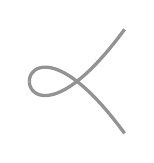
\begin{tikzpicture}
\begin{axis}[hide axis,xmin=-2,xmax=2,ymin=-2,ymax=2,width=4cm]
  \addplot[very thick,domain=-1:0,curveZero,samples=200]{sqrt(x^2+x^3)};%
  \addplot[very thick,domain=-1:0,curveZero,samples=200]{-sqrt(x^2+x^3)};%
  \addplot[very thick,domain=0:1,curveZero]{sqrt(x^2+x^3)};%
  \addplot[very thick,domain=0:1,curveZero]{-sqrt(x^2+x^3)};%
\end{axis}
\end{tikzpicture}
\end{document}

\end{center}
then \(P(x,y)=y^2-x^2\), just the quadratic terms.
\end{example}
Because all terms in \(P(x,y)\) have lowest degree, they have the same degree, so \(P(x,y)\) is homogeneous.
So if we rescale \((x,y)\), we rescale \(P(x,y)\) by some power.
So if \(P(x,y)\) vanishes at some point, it also vanishes at the rescalings \((\lambda x,\lambda y)\) of that point.
So the plane algebraic curve \(0=P(x,y)\) is a union of lines through the origin, i.e. of rescalings.

Rescale \((x,y)\) by a nonzero constant, and then let that constant ``get small'', i.e. look at the powers of that constant, thinking of higher powers as ``smaller''.
Each monomial term rescales by some power of that factor.
Rescale both sides of the equation \(0=p(x,y)\) to get rid of the lowest power.
Intuitively, this means we are ``zooming in'' to see the curve ``through a microscope''.
\begin{example} 
If \(C\) is \(0=x(y^2-x^2-x^3)\), rescaling by a factor \(\lambda\) gives
\[
0=\lambda x\pr{\lambda^2 y^2 - \lambda^2 x^2 - \lambda^3 x^3}.
\]
Divide out the lowest power of \(\lambda\), in this case \(\lambda^3\), to get
\[
0 = x\pr{y^2 - x^2 - \lambda^3 x^3}.
\]
Sending \(\lambda\) to zero, the remaining terms are the homogeneous polynomial \(x\pr{y^2-x^2}\), i.e. exactly the lowest degree terms, exactly our \(P(x,y)\).
\end{example}
After some finite field extension, \(P(x,y)\) splits into homogeneous linear factors, by lemma~\vref{lemma:one.variable.splits}.
The zeroes of this polynomial \(P(x,y)\) form the \emph{tangent lines}\define{tangent line}\define{line!tangent} or \emph{tangents}\define{tangent} to the curve
The number of tangents is at most the degree of the homogeneous polynomial, which is at most the degree of the curve.
The \emph{order}\define{order!of point on curve} of a point \(p_0\) on a curve \(C\) is the number of tangents, counted with multiplicity.
A \emph{regular point}\define{point!smooth}\define{regular!point}\define{point!regular} (also called a \emph{smooth point})\define{point!smooth}\define{smooth!point} of an algebraic curve is a point of order \(1\); any other point is a \emph{singular point}.\define{singular point}\define{point!singular}
A point of order \(2\) is a \emph{double point}\define{double point}\define{point!double}, of order \(3\) a \emph{triple point}\define{triple point}\define{point!triple}, and so on.
A curve without singular points (over the algebraic closure of the field) is \emph{smooth}\define{smooth!curve}\define{curve!smooth} or \emph{regular}.\define{regular!curve}\define{curve!regular}
\begin{problem}{algebraic.curves:fermat}
For every field \(k\) and every integer \(d\ge 1\) not divisible by the characteristic of \(k\), prove that the \emph{Fermat curve}\define{Fermat curve}\define{curve!Fermat} \(F=(x^d+y^d=1)\) is smooth.
\end{problem}
\begin{answer}{algebraic.curves:fermat}
Take some point \((x,y)=(x_0,y_0)\) on \(F\).
Write every point \((x,y)\) of the plane as \((x,y)=(x_0+X,y_0+Y)\) for some \(X,Y\).
The equation of the Fermat curve: \(0=-1+x^n+y^n\) expands out, by the binomial theorem, to
\[
0=-1+x_0^n+nx_0^{n-1}X+\dots+y_0^n+ny_0^{n-1}Y+\dots,
\]
and we then cancel out \(0=-1+x_0^n+y_0^n\) to give
\[
0=n(x_0^{n-1}X+y_0^{n-1}Y)+\dots,
\]
so the linear terms vanish just when \(nx_0^{n-1}=0\) and \(ny_0^{n-1}=0\).
Since the characteristic does not divide \(n\), \(n\ne 0\) in our field, so we divide to find \(0=x_0=y_0\).
But this is not a point of \(F\), since \(x_0^n+y_0^n\) is then not \(1\).
\end{answer}
\begin{problem}{tangents.any.order}
What are the singularities, and their orders, of \(y^p=x^q\) for \(1 \le p, q\), over a field of characteristic not dividing \(p\) or \(q\)?
\end{problem}
\begin{example}
At any regular point, i.e. point of order \(1\), translate variables to put the point at the origin, and linearly change variables to get the tangent line to be the horizontal line \(y=0\).
After a constant rescaling, our equation is \(y=ax^2+bxy+cy^2+\dots\).
Note that we cannot rid our equation of these higher order terms in \(y\).
\end{example}
\begin{example}
A curve of degree \(d\) has at worst a singular point order \(d\).
\end{example}
\begin{example}
The curve \(y^3=x^4\) over the real numbers is the graph of a differentiable (but not polynomial) function \(y=x^{4/3}\).
\begin{center}
\pgfplotsset{compat=1.12,width=4cm}%
\documentclass{standalone}
\usepackage{tikz}
\usepackage{pgfplots}
\usepackage{xparse}
\pgfplotsset{compat=1.14}%
\colorlet{curveZero}{gray!85}
\colorlet{curveOne}{blue!60}
\definecolor{curveOneColor}{rgb}{.6,0,0}
\colorlet{curveTwo}{brown!50!gray}
\colorlet{curveThree}{green!40!gray}
\colorlet{curveFour}{red!50!gray}
\NewDocumentCommand\DrawDotInPlot{O{}mmO{}}%
{%
\fill[gray!15,draw=gray] (axis cs:{#2},{#3}) circle [radius=1.6pt] node[above,black,#4] {\(#1\)};%
}%
\NewDocumentCommand\DrawDot{O{}mmO{}}%
{%
\fill[gray!20,draw=gray] ({#2},{#3}) circle (1.6pt) node[above,black,#4] {\(#1\)};%
}%
\NewDocumentCommand\DrawNode{O{}m}%
{%
\fill[gray!20,draw=gray] (#2) circle (1.6pt) node[above,black] {\(#1\)};%
}%
\NewDocumentCommand\DrawDotThreeD{O{}mmmO{}}%
{%
\fill[gray!20,draw=gray] ({#2},{#3},{#4}) circle (1.6pt) node[above,black,#5] {\(#1\)};%
}%
\colorlet{axisColor}{gray!50}
\tikzstyle{shapeZero}=[fill=curveZero,opacity=.4]
\tikzstyle{shapeOne}=[fill=curveOne,opacity=.4]
\tikzstyle{shapeTwo}=[fill=curveTwo,opacity=.4]
\tikzstyle{shapeThree}=[fill=curveThree,opacity=.4]
\tikzstyle{groupElementLabel}=[minimum size=2.4em]
\tikzstyle{groupElement}=[minimum size=2.4em,shapeZero,draw=curveZero]
\tikzstyle{cosetOne}=[minimum size=2.4em,shapeOne,draw=curveOne]
\tikzstyle{cosetTwo}=[minimum size=2.4em,shapeTwo,draw=curveTwo]


\begin{document}
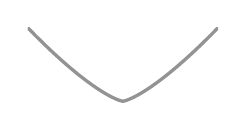
\begin{tikzpicture}
\begin{axis}[hide axis,xmin=-1,xmax=1,ymin=-1,ymax=1,width=4cm]
  \addplot[very thick,domain=-1:1,curveZero,samples=300]{abs(x)^(4/3)};%
\end{axis}
\end{tikzpicture}
\end{document}

\end{center}
Its tangents at the origin arise from keeping the lowest degree homogeneous terms: \(y^3=0\), i.e. there is a unique tangent \(y=0\).
Nonetheless, over the complex numbers this curve is \emph{not} the graph of a differentiable complex function of a complex variable.
\end{example}
The tangents are just the lines on which the linear factors vanish, say
\[
P(x,y)=(a_1x+b_1y)^{n_1}\dots(a_2x+b_2 y)^{n_k},
\]
with the nonzero linear factors \(a_ix+b_i y\) each vanishing on a different tangent \(a_ix+b_iy=0\).
Each power \(n_i\) is the \emph{multiplicity}\define{multiplicity!tangent line}\define{tangent line!multiplicity} of its associated tangent line \(ax_i+by_i=0\).
A \emph{simple tangent}\define{simple!tangent line}\define{tangent line!simple} is one of multiplicity one.
\begin{example}
At the origin, the curve \(0=y^4-x^4y-xy^3+x^5\) has homogeneous lowest terms \(y^4-xy^3=y^3(y-x)\):
\[
\begin{array}{rll}
\toprule
\text{Tangent line}&\text{Multiplicity}&\text{Terminology}\\
\cmidrule(r){1-1}\cmidrule(lr){2-2}\cmidrule(l){3-3}
y=x&1&\text{simple}\\
y=0&3\\
\bottomrule
\end{array}
\]
\end{example}
\begin{problem}{algebraic.curves:find.tangents}
Find the tangents and their multiplicities at the origin for
\begin{enumerate}
\item
\((x^2+y^2)^2+3x^2y-y^3\)
\item
\((x^2+y^2)^3-4x^2y^2\)
\item
\((x^2+y^2)^4+x^{1000}\)
\end{enumerate}
\end{problem}
Write the derivatives of a function \(f(x,y)\) as \(f_x,f_y\) to mean
\[
f_x=\frac{\partial f}{\partial x}, 
f_y=\frac{\partial f}{\partial y},
\]
and higher derivatives as
\[
f_{xx}=\frac{\partial^2 f}{\partial x^2},
f_{xy}=\frac{\partial^2 f}{\partial x\partial y},
\]
and so on.
Expanding out in powers, clearly the singularities of a curve \(C=(0=f(x,y))\) occur just where the derivatives \(f_x\) and \(f_y\) vanish: the linear approximations of the polynomial.
\begin{example}
Let's find the singular points of \(C=(x^3+y^3-3x^2-3y^2+3xy+1)\) over any field not of characteristic \(2\) or \(3\):
\begin{align*}
p(x,y)&=x^3+y^3-3x^2-3y^2+3xy+1,\\
\pderiv{p}{x}&=3x^2-6x+3y,\\
\pderiv{p}{y}&=3y^2-6y+3x.
\end{align*}
To have these vanish, vanishing of \(\pderiv{p}{x}\) gives \(y=2x-x^2=x(2-x)\).
By symmetry, vanishing of \(\pderiv{p}{y}\) then gives \(x=y(2-y)\).
Plugging one into the other gives
\[
\begin{array}{ccc}
\toprule
x&y&p(x,y)\\
\cmidrule(r){1-1}\cmidrule(lr){2-2}\cmidrule(l){3-3}
0&0&1\\
1&1&0\\
-\frac{\sqrt{3}i}{2}&\frac{\sqrt{3}i}{2}&1\\
\frac{\sqrt{3}i}{2}&-\frac{\sqrt{3}i}{2}&1\\
\bottomrule
\end{array}
\]
So we only have to look at the point \((x,y)=(1,1)\).
Changing variables to \(X=x-1, Y=y-1\), so \(x=X+1, y=Y+1\), we find
\[
p(x,y)=X^3 + Y^3 + 3XY.
\]
So the lowest order terms are \(3XY=3(x-1)(y-1)\), simple tangents \(X=0\) and \(Y=0\), i.e. \(x=1\) and \(y=1\), an ordinary double point.
\begin{center}
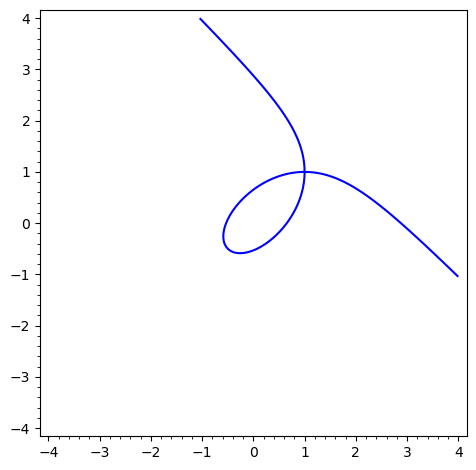
\includegraphics[width=4cm]{node}
\end{center}
\end{example}
\begin{problem}{algebraic.curves:Hasse.curve}
A \emph{symmetric cubic curve}\define{symmetric cubic curve}\define{curve!symmetric cubic}\define{cubic curve!symmetric} is a plane algebraic curve with equation
\[
x^3+y^3+1=3axy.
\]
Over a field not of characteristic \(3\), prove that the symmetric cubic curve is smooth if \(a^3\ne 1\).
\end{problem}
\begin{answer}{algebraic.curves:Hasse.curve}
Homogenize to
\[
0=x^3+y^3+z^3-3axyz.
\]
Differentiate to find
\[
x^2=ayz, y^2=axz, z^2=axy.
\]
Multiply the first equation by \(x\), the second by \(y\), the third by \(z\): 
\[
x^3=y^3=z^3=axyz.
\]
Multiply these together
\[
x^3y^3z^3=a^3x^3y^3z^3.
\]
So \(x=0\) or \(y=0\) or \(z=0\) or \(a^3=1\).
If \(x=0\), then \(y^2=axz=0\) and \(z^2=axy=0\), impossible since \(x,y,z\) can't all vanish for a point of the projective plane.
Similarly if \(y=0\) or if \(z=0\).
So finally \(a^3=1\).
\end{answer}
\begin{example}
Some examples of symmetric cubic curves, for various real values of \(a\); the straight line is at \(a=1\):
\begin{center}
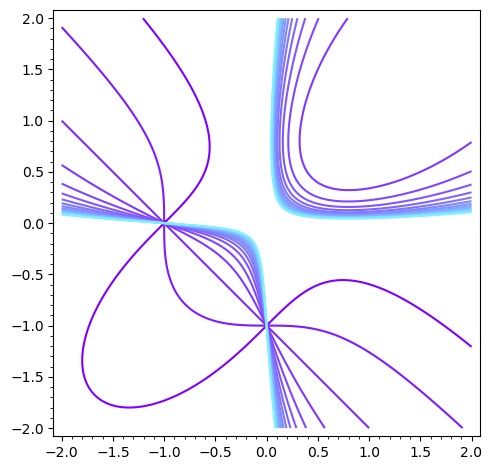
\includegraphics[width=4cm]{symmetric-cubics.png}
\end{center}
\end{example}
\begin{problem*}{algebraic.curves:Hasse.singular}
Prove that every symmetric cubic curve 
\[
x^3+y^3+1=3axy
\]
with \(a^3=1\) is a union of three lines.
\end{problem*}
\begin{theorem}
Every nonsingular plane algebraic curve is irreducible.
\end{theorem}
\begin{proof}
Take a reducible plane algebraic curve and write it as a union of irreducible component curves.
Correspondingly, write its equation as a product of two polynomials.
Any two of the irreducible components intersect somewhere (at least in the points defined over the algebraic closure of the field), say at a point \(p\).
Translate the picture to arrange that \(p\) is the origin.
Each of the two components has equation given by a polynomial vanishing at the origin, so the original curve is a product of such polynomials.
Therefore the equation of the reducible curve vanishes to at least second order.
Therefore every reducible curve is singular.
\end{proof}
\begin{example}
Look at the Fermat curve: there are smooth curves of all degrees (except maybe those degrees divisible by the characteristic of the field), and these are therefore irreducible.
\end{example}
\begin{theorem}
Every irreducible curve has only finitely many singularities.
\end{theorem}
\begin{proof}
Take an irreducible curve \(C=(0=f(x,y))\), say of degree \(d\).
There are only at most \(d(d-1)\) values of \(x\) at which \(f_x\) vanishes, unless \(f,f_x\) have a common factor, by proposition~\vref{proposition:resultant.degree}; the same is true of \(f_y\).
Since \(f\) is irreducible, any common factor has to be \(f\), up to constant multiple.
But \(f_x,f_y\) have lower degree than \(f\); being multiples of \(f\) ensures they both vanish.
So to have more than \(d^2(d-1)^2\) singular points, \(f_x\) and \(f_y\) both vanish everywhere.
If the characteristic of the field is zero, this ensures that \(f\) is a constant, so \(C\) is not a curve.
Suppose the characteristic of the field is a prime \(p\).
Expand out \(f\) to find that vanishing of \(f_x,f_y\) is precisely that every term in \(f\) is a pure \(p^{\text{th}}\) power:
\[
f(x,y)=a_{00}+a_{10}x^p+a_{01}y^p+a_{11}x^py^p+\dots
\]
with finitely many terms in all.
Take a finite degree extension field in which each \(a_{jk}\) is itself a \(p^{\text{th}}\) power, say \(a_{jk}=b^p_{jk}\).
Note that in our field, because it has characteristic \(p\), the Frobenius morphism \(\alpha\mapsto\alpha^p\) is an automorphism of fields; see lemma~\vref{lemma:Frobenius}.
We can thus write \(f(x,y)=g(x,y)^p\) where
\[
g(x,y)=b_{00}+b_{10}x+b_{01}y+b_{11}xy+\dots
\]
Hence our curve is not irreducible.
\end{proof}

\section{Formal power series}
\begin{corollary}
At any smooth point of a plane algebraic curve, we can arrange by a linear change of variables that the curve passes through the origin of coordinates, and is not tangent to the vertical coordinate axis there.
Then the equation of the curve \(0=p(x,y)\) has a unique formal power series solution \(y=y(x)\) at that point.
\end{corollary}
\begin{problem}{formal.power.series:reduce.curve}
Prove that the polynomial \(p(x,y)=y^2-x^2(1+x)\) is irreducible as a polynomial over any commutative ring with identity.
(Hint: a stronger result is perhaps easier: \(y^2-f(x)\) is irreducible just when the polynomial \(f(x)\) is a square.)
Over the real numbers, its zeroes form a plane algebraic curve:
\begin{center}
\pgfplotsset{compat=1.12,width=7cm}%
\documentclass{standalone}
\usepackage{tikz}
\usepackage{pgfplots}
\usepackage{xparse}
\pgfplotsset{compat=1.14}%
\colorlet{curveZero}{gray!85}
\colorlet{curveOne}{blue!60}
\definecolor{curveOneColor}{rgb}{.6,0,0}
\colorlet{curveTwo}{brown!50!gray}
\colorlet{curveThree}{green!40!gray}
\colorlet{curveFour}{red!50!gray}
\NewDocumentCommand\DrawDotInPlot{O{}mmO{}}%
{%
\fill[gray!15,draw=gray] (axis cs:{#2},{#3}) circle [radius=1.6pt] node[above,black,#4] {\(#1\)};%
}%
\NewDocumentCommand\DrawDot{O{}mmO{}}%
{%
\fill[gray!20,draw=gray] ({#2},{#3}) circle (1.6pt) node[above,black,#4] {\(#1\)};%
}%
\NewDocumentCommand\DrawNode{O{}m}%
{%
\fill[gray!20,draw=gray] (#2) circle (1.6pt) node[above,black] {\(#1\)};%
}%
\NewDocumentCommand\DrawDotThreeD{O{}mmmO{}}%
{%
\fill[gray!20,draw=gray] ({#2},{#3},{#4}) circle (1.6pt) node[above,black,#5] {\(#1\)};%
}%
\colorlet{axisColor}{gray!50}
\tikzstyle{shapeZero}=[fill=curveZero,opacity=.4]
\tikzstyle{shapeOne}=[fill=curveOne,opacity=.4]
\tikzstyle{shapeTwo}=[fill=curveTwo,opacity=.4]
\tikzstyle{shapeThree}=[fill=curveThree,opacity=.4]
\tikzstyle{groupElementLabel}=[minimum size=2.4em]
\tikzstyle{groupElement}=[minimum size=2.4em,shapeZero,draw=curveZero]
\tikzstyle{cosetOne}=[minimum size=2.4em,shapeOne,draw=curveOne]
\tikzstyle{cosetTwo}=[minimum size=2.4em,shapeTwo,draw=curveTwo]


\begin{document}
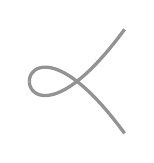
\begin{tikzpicture}
\begin{axis}[hide axis,xmin=-2,xmax=2,ymin=-2,ymax=2,width=4cm]
  \addplot[very thick,domain=-1:0,curveZero,samples=200]{sqrt(x^2+x^3)};%
  \addplot[very thick,domain=-1:0,curveZero,samples=200]{-sqrt(x^2+x^3)};%
  \addplot[very thick,domain=0:1,curveZero]{sqrt(x^2+x^3)};%
  \addplot[very thick,domain=0:1,curveZero]{-sqrt(x^2+x^3)};%
\end{axis}
\end{tikzpicture}
\end{document}

\end{center}
Explain how to factor \(p(x,y)\) into a product of two formal power series, each linear in \(x\) (so it is \emph{not} irreducible as a formal power series), over any commutative ring with identity.
Roughly speaking, near the origin, the plane algebraic curve consists of the ``graphs'' of two ``functions'', but the ``functions'' might just be formal power series.
\end{problem}
\begin{answer}{formal.power.series:reduce.curve}
If \(y^2-f(x)\) is reducible, each factor is linear in \(y\), or else one is constant in \(y\) and the other quadratic.
In the second case: the factor constant in \(x\) is multiplied by a quadratic in \(x\), coefficients polynomial in \(y\), giving \(x^2+\dots\), constant in \(y\), so the factor constant in \(x\) and \(y\).
In the first case: each linear factor has, up to rescaling, a unit coefficient in front of \(x\)
\[
x^2-f(y)=(x+b(y))(x+c(y))=x^2+x(b(y)+c(y))+b(y)c(y),
\]
so that \(c(y)=-b(y)\), and then \(x^2-f(y)=x^2-b(y)^2=(x+b(y))(x-b(y))\).
Clearly \(y^2(1+y)\) is not a square, because it has odd degree.
But over formal power series,
\[
x^2-y^2(1+y)=(x-y\sqrt{1+y})(x+y\sqrt{1+y})
\]
where \(\sqrt{1+y}\) means that we apply our previous results to construct the unique square root of \(1+y\) for which we take \(\sqrt{1}\) to be \(1\).
\end{answer}
Given an algebraic curve \(0=p(x,y)\), we want to write out a Puiseaux series \(y=y(x)\) to ``solve''  the equation \(0=p(x,y)\), and we want to consider both the existence and the uniqueness of this series.
We already see that there is no such formal power series in integer powers of \(x\).
We will not prove:
\begin{theorem}[Newton--Puiseaux]\define{theorem!Newton--Puiseaux}\define{Newton--Puiseaux theorem}
Take a plane algebraic curve over an algebraically closed field \(k\).
For simplicity, we suppose that the origin lies on the curve, and that the curve is irreducible.
There is a Puiseaux series \(y(x)\) so that \(0=p(x,y(x))\), in the ring 
of Puiseaux series.
The number of distinct such series agrees with the order of the origin as a point of the algebraic curve.
\end{theorem}

\section{Parameterization}
If we work with rational functions, not formal power series, we might not be able to solve the equation of a curve, but we can come close.
A \emph{local parameter} for a curve \(C\) near a point \(p_0=(x_0,y_0)\) of \(C\) is a rational function \(t\) regular near \(p_0\) so that \(t(x_0,y_0)=0\) and so that, for any rational function \(f\) which is not everywhere zero on any component of \(C\) containing \(p_0\), \(f=t^k F\) for some integer \(k\) and rational function \(F\) regular at \(p_0\) with \(F(p_0)\ne 0\), and so that \(k\ge 0\) just when \(f\) is regular at \(p_0\).
\begin{problem}{algebraic.curves:local.param}
Prove that any two local parameters \(t,T\) for \(C\) at \(p_0\) have ratio \(t/T\) regular and nonzero near \(p_0\).
\end{problem}
\begin{answer}{algebraic.curves:local.param}
\(T=t^k F\) for some \(F\ne 0\) regular near \(p_0\), and reciprocally \(t=T^{\ell} G\) for some \(G\ne 0\) regular near \(p_0\).
Being both regular, \(k,\ell\ge 0\).
So \(T=t^k F=T^{k\ell} G^k F\), and uniqueness forces \(k\ell=1\) so \(k=\ell=1\).
\end{answer}
\begin{theorem}
Every plane algebraic curve has a local parameter near any smooth point.
\end{theorem}
\begin{proof}
After a constant rescaling, our equation is \(y=ax^2+bxy+cy^2+\dots\).
We will try to take \(t(x,y)\defeq x\).
Gathering up all the pure \(x\) terms, write this as
\[
y=xX(x)+y(bx+cy+\dots),
\]
We try again to solve for \(y\):
\[
y(1-bx-cy+\dots)=xX(x),
\]
and so
\[
y=\frac{xX(x)}{1-bx-cy+\dots}
\]
which we write as \(y=xY(x,y)\), where \(Y(x,y)\) is regular at the origin.

Take any rational function \(f(x,y)\) vanishing at the origin:
\[
f(x,y)=\frac{p(x,y)}{q(x,y)}, 
\]
so \(p(0,0)=0\) and \(q(0,0)\ne 0\).
Plug in: on our curve
\[
f(x,y)=f(x,xY(x,y))=\frac{p(x,xY(x,y)}{q(x,xY(x,y))}.
\]
Since \(p(0,0)=0\), \(p(x,xY(x,y))\) has a factor of \(x\), say 
\[
p(x,xY(x,y))=xr(x,y),
\]
with \(r(x,y)\) regular on our curve near the origin.
So on the curve
\[
f(x,xY(x,y))=x\frac{r(x,y)}{q(x,xY(x,y))}=xF(x,y),
\]
with \(F(x,y)\) regular at the origin.
If \(F(0,0)=0\), repeat this argument to write \(F(x,xY(x,y))=xF_1(x,y)\), and so on.
So eventually \(f=x^k F\) for some \(F\) regular at the origin and not zero, and similary \(p=x^k P\) for some \(P\) regular at the origin and not zero.
We need to see that there is only one possible value of \(k\) that can occur.

Write our curve's equation \(y=ax^2+bxy+cy^2+\dots\) as a polynomial \(b(x,y)\) in the plane.
As polynomials in \(y\), with coefficients rational functions of \(x\), compute B\'ezout coefficients \(s(x,y),t(x,y)\) for \(b(x,y),p(x,y)\), with greatest common divisor \(1\) because they have no common factor.
Scale both sides by a least common denominator polynomial in \(x\) to find :
\[
s(x,y)b(x,y)+t(x,y)p(x,y)=g(x),
\]
for some polynomial \(g(x)\).
Factor as much \(x\) out the greatest common divisor as possible, say
\[
g=x^{\ell}G.
\]
so \(G(0)\ne 0\).
Then \(tp=x^{\ell}G\) on our curve.
But \(p=x^kP\), i.e. \(x^{k-\ell}tP=G\).
If \(k>\ell\), this makes \(G\) vanish at the origin.
If \(k<\ell\), \(tP=Gx^{\ell-k}\) makes \(P\) vanish at the origin.
\end{proof}

\section{Ideals}
\begin{example}
Given a plane algebraic curve \(C\) and a point \(p_0 \in C\) (say, to be precise, that \(p_0 \in C(k)\) is a point defined over \(k\)), we are naturally interested in the regular functions on \(C\) vanishing at \(p_0\).
If \(p_0\) has coordinates \(p_0=\pr{x_0,y_0}\), then the polynomial functions \(x-x_0, y-y_0\) vanish simultaneously only at \(p_0\).
For simplicity, translate the plane so that \(p_0\) lies at the origin.
A regular function on \(C\) vanishes at \(p_0\) just when it is a sum \(xg(x,y)+yh(x,y)\), since every polynomial function vanishing at the origin is expressible in a finite Taylor series expansion.
In other words, the regular functions on \(C\) vanishing at the origin are precisely the ideal \(I=(x,y)\). 
\end{example}
\begin{example}
Similarly, the regular functions on \(C\) vanishing at \(\pr{x,y}=p_0=\pr{x_0,y_0}\) are the polynomials of the form \(\pr{x-x_0}g(x,y)+\pr{y-y_0}h(x,y)\), so constitute the ideal \(I=\pr{x-x_0,y-y_0}\).
This \(I\) is the kernel of the morphism \(p(x,y) \mapsto p\of{x_0,y_0}\), mapping \(k[C] \to k\).
\end{example}
This is the motivation for the name ``ideal'': an ideal is like a idealized notion of a point.
\begin{example}
The regular functions on the real number line are the polynomials \(p(x)\), and those which vanish at a point \(x=x_0\) are those of the form \(\pr{x-x_0}p(x)\).
Similarly, if we take two points \(x_0 \ne x_1\), then the regular functions on the line vanishing at both points are the polynomials of the form \(\pr{x-x_0}\pr{x-x_1}p(x)\), the polynomials divisible \(\pr{x-x_0}\pr{x-x_1}\).
\end{example}
\begin{example}
If we imagine running the two points into one another, so that they collide at \(x=0\), then these polynomials approach polynomials divisible by \(x^2\).
We could think of the equation \(x^2=0\), or of the ideal \(I=\pr{x^2}\), as representing a ``double point''.
\end{example}
\begin{example}
Working over \(k\defeq\Q{}\) on the curve \(C\defeq(x^2=y)\), the ideal \(I\defeq(x-2)\) does not correspond to any point of \(C\) defined over \(k\).
Again, we can think of \(I\) as an ``ideal point''.
\end{example}
\begin{problem}{algebraic.curves:reg.fns}
Prove that a polynomial \(p(x,y)\) vanishes as a regular function on some irreducible plane algebraic curve \(C=(c(x,y)=0)\) just when \(c(x,y)\) divides \(p(x,y)\).
\end{problem}
\begin{answer}{algebraic.curves:reg.fns}
If \(c(x,y)\) divides \(p(x,y)\), clearly \(p(x,y)=0\) on every \(\bar{k}\)-point where \(c(x,y)=0\).
Suppose that \(p(x,y)=0\) on those points.
For any constant value of \(x\) or \(y\) in \(\bar{k}\), there are points where \(c(x,y)=0\) and so the resultant of \(p(x,y),c(x,y)\) in the other variable vanishes.
So the resultant vanishes for infinitely many values, so vanishes everywhere.
So \(p(x,y),c(x,y)\) have a common factor in \(k[x,y]\).
Recall that \(c(x,y)\) is irreducible.
\end{answer}
\begin{example}
The surface \(S=(x^2+y^2=z^2)\) over \(\R{}\) is a cone.
The subset of \(S\) cut out by the equation \(z=1\) is a circle on that cone, a curve on the surface.
The subset of \(S\) cut out by the equation \(z^2+1=0\) is empty, but has complex points. 
Even over the real numbers, we have an ideal \(I=(z^2+1)\subset\R{}[S]\), which we can think of as a kind of ``ideal curve''.
So intuitively, ideals represent ``ideal geometric objects'', which perhaps we can't really draw.
\end{example}

\section{Sage}
Sage can usually plot the real points of a plane algebraic curve.
For any equation like \(y^3+x^3-6x^2y=0\) the code 
\begin{sageblock}
x,y=var('x,y')
contour_plot(y^3+x^3-6*x^2*y==0, (x,-10,10), (y,-10,10)) 
\end{sageblock}
yields a picture of the level sets of the function \(y^3+x^3-6x^2y\):
\begin{center}
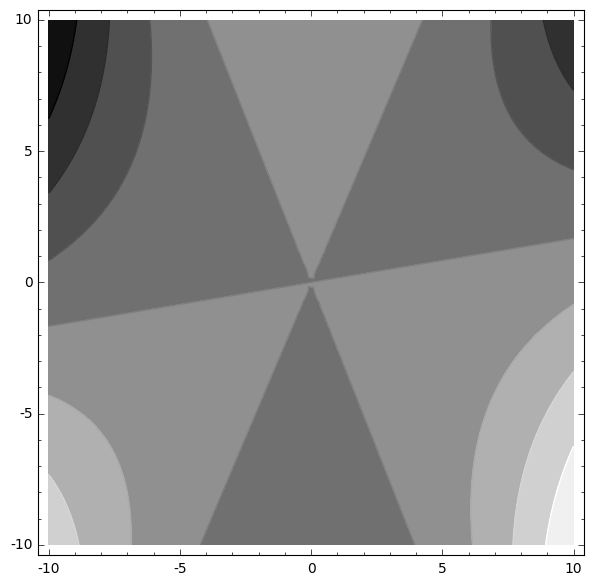
\includegraphics[width=5cm]{sage-algebraic-curve-plot}
\end{center}
from which we can see that our curve is a union of three lines.
Similarly
\begin{sageblock}
x,y=var('x,y')
contour_plot(y^2-x*(x-1)*(x-2)==0, (x,-3,4), (y,-5,5))
\end{sageblock}
yields level sets like
\begin{center}
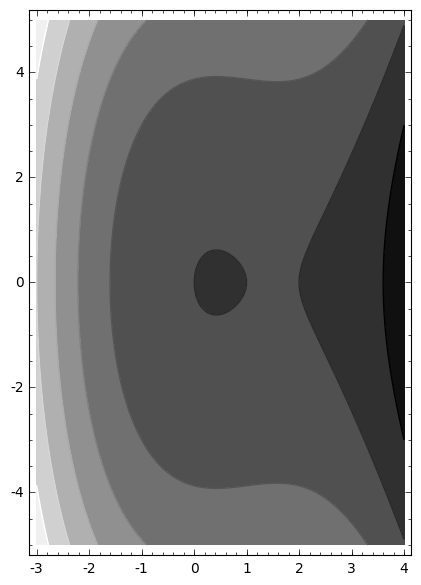
\includegraphics[width=5cm]{sage-algebraic-curve-plot-2}
\end{center}
and we can also plot the plane algebraic curve, without the other level sets, using
\begin{sageblock}
f(x,y) = y^2-x*(x-1)*(x-2)
implicit_plot(f, (-3, 4), (-5, 5))
\end{sageblock}
yielding
\begin{center}
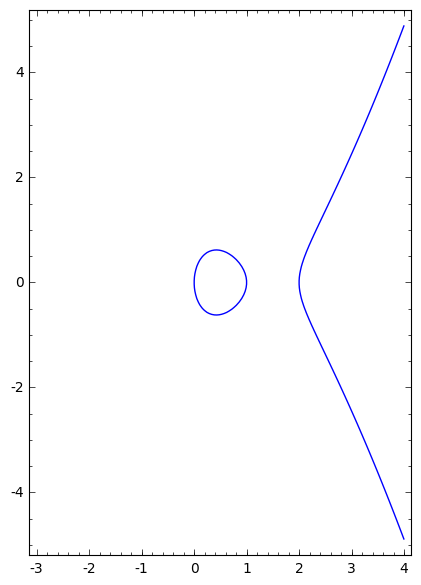
\includegraphics[width=5cm]{sage-algebraic-curve-plot-3}
\end{center}
Similarly, we can draw algebraic surfaces in space:
\begin{sageblock}
f(x,y,z) = y^2-x*(x-1)*(x-2)+z^4-1
implicit_plot3d(f, (-3, 4), (-5, 5), (-1,1))
\end{sageblock}
yielding
\begin{center}
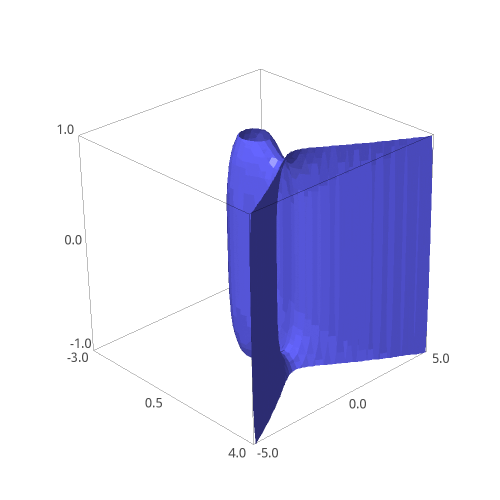
\includegraphics[width=5cm]{sage-algebraic-surface-plot}
\end{center}
